\partsintesi{Activitats de síntesi}{Activitats de síntesi}



\begin{mylist}
 
	
	 \exer[2] Efectua les operacions:
	
	\begin{tasks}(2)
		\task $\frac{5}{4}-\left(\frac{3}{2}-\frac{1}{4}\mathrm{:}\frac{-3}{2}\right)=$ 
		\task $\frac{\ofrac{2}{5}- \left(\ofrac{3}{2}:\ofrac{8}{5}\right)^{-1}}{2-\left(\ofrac{2}{3}\right)^{2}}=$
	\end{tasks}
	\answers{ a) $\frac{-5}{12}$;\quad b) $\frac{-3}{7}$}
	
	\exer[2]  Expressa com a potència única ${\left[5^2 \cdot 25^2 \right]}^3 : 5^{-2}=$
 	\answers{ $5^{20}$}
 
 	
	 \exer[2] Un estudiant de 3r d'ESO es proposa el dia 1 de setembre repassar matemàtiques durant una quinzena, fent cada dia 2 exercicis més que el dia anterior. Si el primer dia va començar fent 1 exercici, quants d'exercicis va fer dia 15? Quants exercicis va fer en total?
	 	\answers{a) 29 exercicis dia 15; \par b) 225 exercicis en total.}
 
 	
	 \exer[2] El nombre de vegades que un grup d'alumnes de 3r ESO ha anat al cinema el darrer mes ve donat  per la següent taula:
	 
	 \answers{ a) $N=25$; $\sum f_i x_i = 41$; $\sum f_i x_i^2 =83$;\par c) $Mo=2$; $\bar x=1,64$; $\sigma=0,79$; $CV=0,48$ (48 \%).}
	\begin{enumerate}
		\item Completa la taula

	\begin{tabular}{|p{1.2in}|p{1.2in}|p{1.2in}|p{1.2in}|} \hline 
	 \rowcolor{lightgray}	\textbf{ $x_i$ -- pics al cine} & \textbf{$f_i$ -- n. alumnes} & $f_i \cdot x_i$ & $f_i \cdot x_i^2$ \\ \hline 
		0 & 2 &  &   \\ \hline 
		1 & 8 &  &  \\ \hline 
		2 & 12 &  &  \\ \hline 
		3 & 3 &  &  \\ \hline 
		\rowcolor{lightgray} \textbf{SUMES} & \textbf{N=} & $\sum f_i x_i$= & $\sum f_i x_i^2$= \\ \hline 
	\end{tabular}
	
	\item Representa un diagrama de barres. 
	
\item Calcula la Moda (Mo),  Mitjana Aritmètica ($\bar x$) ,  la Desviació Típica ($\sigma$)  i el  coeficient de Variació (CV)  de la variable.
		\end{enumerate}
	
	 
	
	\exer[2] Una urna té 3 bolles blanques i 7 negres. Extreim dues bolles amb reemplaçament. Fes un diagrama d'arbre. Trobau la probabilitat de treure:
	\begin{tasks}(2)
		\task almenys una bolla blanca
		\task les dues bolles de diferent color
	\end{tasks} 
	\answers{ a) 0,51; b) 0,42}
 
	\exer[2] Donats els polinomis : $p(x)=3x^4+7x^3-3x^2+3x-6$, $q(x)=-2x^3+5x^2-7x-1$i $r(x)=2x+3$, calculau:
	\begin{tasks}(4)
		\task $p(x)+q(x)+r(x)$
		\task $p(x)-q(x)$
		\task $q(x)\cdot r(x)$
		\task $r(x)^2$
	\end{tasks}
\answers{ a) $3x^4+5x^3+2x^2-2x-4$; \par b) $3x^4+9x^3-8x^2+10x-5$; \par c) $-4x^4+4x^3+x^2-23x-3$; \par d) $4x^2+12x+9$}
	 
	 \exer[2] Resol les equacions:
	\begin{tasks}(2)
		\task $\frac{x\cdot (x+2)}{3}=x+\frac{1}{2}$  
		\task ${(x-2)}^2=9$
	\end{tasks} 
\answers{  a) $x=1,82$ i $x=-0,82$; \par b) $x=-1$ i $x=5$}
	
	\exer[2] Resol el sistema pel mètode més adient: $\left \{ \begin{array}{c}
	2x+y=1 \\ 
	y+3x=-2 \end{array}
	\right.$ 
	\answers{ $x=-3$ i $y=7$}
	
	\exer[2] Dues màquines funcionant 6 hores consumeixen 1500 kWh. Quant consumiran 3 màquines funcionant 8 hores?
	\answers{ Consumeixen $3000$ kWh}
	
	\exer[2] Pel lloguer d'un cotxe cobren 100 \euro\ \ diaris més 0.30 \euro\ \ per kilòmetre recorregut. Troba l'equació que relaciona els kilòmetres i el preu i representa-la. Si un dia s'han fet 300 km, quant s'haurà de pagar? Si un altre dia vàrem pagar 119,5 \euro\ \, quants kilòmetres varem fer?
	\answers{  $y=0.30 \cdot x + 100$; \quad $y=190$ €; \quad $x=65$ km}
	
	 
	
	 \exer[2] Calcula el vèrtex i representa gràficament la paràbola $y=-x^2+5x-2$.
	 \answers{ Paràbola convexa en vèrtex al punt $x=5/2$, $y=17/4$}
	 
 	
		\exer[2]  Sabem que per trobar el nombre \textit{x} que està enmig de dos donats \textit{a} i \textit{b}, basta calcular la seva mitjana $\overline{x}=\frac{a+b}{2}$. Quin és el nombre que està en enmig de 1.8585··· i 2.888····.\textit{Ajuda: Passa cada nombre a fracció i opera les fraccions.}
	\answers{  $1.8585\cdots= \frac{184}{99}$  i $2.888 \cdots= \frac{26}{9}$. La mitjana  és $x=\frac{235}{99}$. }
	
	\vspace*{-1.5cm}
	\exer[2] \begin{minipage}[t]{0.7\textwidth}
		A na Marta li descompten la cinquena part del sou en concepte de \textit{IRPF} i la sisena part per a la \textit{Seguretat Social}. Si sabem que cobra 600 \euro\ \ nets, quin és el seu sou brut? \textit{Ajuda: Comença comprovant que després dels descomptes només li queden les 19/30 parts del sou.}
	\end{minipage}
	\begin{minipage}{0.3\textwidth}
		\centering
		\vspace{1.5cm}
		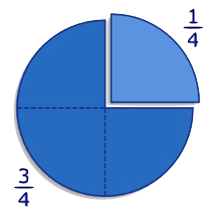
\includegraphics[width=0.5\textwidth]{sintesi/image1}
	\end{minipage}
	 \answers{  947,37 \euro{} \ de sou brut}
	
 \vspace{-1.5cm}
 \exer[2] \begin{minipage}[t]{0.7\textwidth}
 	 Contesta:
 	 \begin{tasks}
 	 	\task La mida d'un bacteri 0,00000247 en notació científica.
 	 	\task El valor decimal de $\sqrt[6]{7,2\cdot {10}^{-3}}$
 	 	\task  El que mesura un costat d'un cub de volum 125 cm${}^{3}$. Recorda $V=c^3$
 	 \end{tasks}
 \end{minipage}
 \begin{minipage}{0.3\textwidth}
 	\centering
 	\vspace{1.5cm}
 	
\includegraphics[width=0.5\textwidth]{sintesi/image2}
 \end{minipage}
 	\answers{  a) $2,47\cdot 10^{-6}$   \quad b) $0,43943\cdots$ \quad c) 5 cm perquè $5^{3}$=125}
 
	
 
	
	
		\exer[2]  Calcula la teva edat en segons expressada en notació científica.
	\answers{ Per exemple, 17 anys = $5,36\cdot 10^{8}$ s}
	
	
  \vspace{-1.25cm}
  \exer[2] \begin{minipage}[t]{0.7\textwidth}
  	Una nedadora va entrenar tots els dies durant tres setmanes. El primer dia va nedar 15 minuts, i cada dia nedava 5 minuts més que el dia anterior. Quant de temps va nedar l'últim dia? I durant de les tres setmanes?  
  \end{minipage}
  \begin{minipage}{0.3\textwidth}
  	\centering
  	\vspace{1.5cm}
  	
\includegraphics[width=0.5\textwidth]{sintesi/image3}
  \end{minipage}
\answers{El dia 21 va nadar 115 minuts; durant els 21 dies va nadar 1365 minuts.}
  
	\pagebreak
	\mbox{}
	  \vspace*{-1.75cm} 
	\exer[2] \begin{minipage}[t]{0.7\textwidth}
		  El número d'estrelles dels hotels d'una ciutat és:
		  \vspace{0.25cm}
		\begin{center}
		\begin{tabular}{c c c c}
		3, 3, 4, 3, 4  & 3, 1, 3, 4, 3  & 3, 3, 2, 1, 3  & 3, 3, 2, 3, 2 \\
		2, 3, 3, 3, 2  & 2, 2, 2, 2, 3 &  2, 1, 1, 1, 2 &  2, 4, 1 \\
		\end{tabular}
		\end{center}
	\end{minipage}
	\begin{minipage}{0.3\textwidth}
		\centering
		\vspace{1.5cm}
		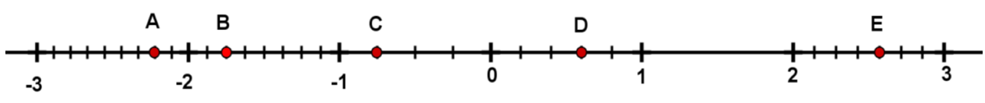
\includegraphics[width=0.5\textwidth]{sintesi/image4}
	\end{minipage}
		\vspace{-0.5cm}
	\begin{tasks}
		\task Quants hotels té la ciutat en total?
		\task Construeix una taula de freqüències i un diagrama de barres.
		\task  Calcula la mitjana, la desviació típica i el coeficient de variació de la variable.
	\end{tasks}
\answers{  a) 38 hotels; c) mitjana=2.47; desv. típica=0.88;  C.V. = 0.36 (36\%)}	
	
	 
	
	\exer[2]  Contesta:
	\begin{tasks}
		\task  Quin és el grau de $-5xyz^2$?
		\task  Simplifica  $7x^2\cdot \ 2x\ -\ x\cdot \left(2\ x^2+\ 5\ x^5:x^3\right)=$
		\task  Efectua l'operació ${\left(x-2\right)}^2+\ \left(x+2\right)\cdot \left(x-2\right)=$
	\end{tasks}
	\answers{  a) grau 4;   \quad  b)  $7x^{3}$;   \quad  c) 2 $x^{2}-4x$}
	
	
 \vspace{-1.5cm}
 \exer[2] \begin{minipage}[t]{0.7\textwidth}
 	Una urna conté 6 bolles blaves i 6 de vermelles. Es mescla el seu contingut i s'extreuen dues bolles \textbf{\underbar{sense reemplaçament}}. Quina és la probabilitat que surtin dues bolles de diferent color? \textit{Ajuda: Fes un diagrama d'arbre.}
 \end{minipage}
 \begin{minipage}{0.3\textwidth}
 	\centering
 	\vspace{1.5cm}
 	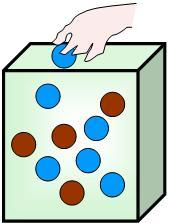
\includegraphics[width=0.5\textwidth]{sintesi/image5}
 \end{minipage}
 \answers{  $P=6/11 \approx 0,54$}
	
	  
	\vspace{-1.5cm}
	\exer[2] \begin{minipage}[t]{0.7\textwidth}
		 A l'aula de 3r A hi ha doble nombre d'alumnes que a l'aula de 3r B. A més es sap que, si es passen 8 alumnes de 3r A a 3r B, les dues aules tindran el mateix nombre d'alumnes. Quants alumnes hi ha en cadascuna d'aquestes aules? \textit{Ajuda: Planteja i resol un sistema d'equacions}
	\end{minipage}
	\begin{minipage}{0.3\textwidth}
		\centering
		\vspace{1.5cm}
		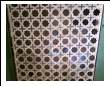
\includegraphics[width=0.5\textwidth]{sintesi/image6}
	\end{minipage}
	\answers{   $x=2y$;  $x -8 = y+8$;  \quad 3r A: $x= 32$; \quad 3r B: $y=16$.}
	
		
		\exer[2]  Resol, si és possible, les següents equacions:
		\begin{tasks}(4)
			\task $x^2+\ 4\ =\ 0$
			\task ${\ \ x}^2-\ 9\ =\ 0$
			\task $ x^2+\ 2x\ =0$
			\task $ x^2+\ 2x-3\ =\ 0$
		\end{tasks} 
		\answers{  a) No té solució;  \quad    b) $x=-3$ i $x=3$;     \par  c) $x=0$ i $x=-2$;  \quad    d) $x=1$   i   $x=-3$}
	
		\exer[2]  D'aquí a 30 anys l'edat de Pere serà la cinquena part del quadrat de l'edat actual. Calcula l'edat actual d'en Pere. \textit{Ajuda: Planteja i resol una equació de 2n grau.}
	  \answers{    $x+30=\frac{x^2}{5}$;  $x^2-5x-150=0$  $\rightarrow$ $x=-10$ no val;  $x=15$ anys.}
	
	
		\exer[2] Nou persones han gastat en transport 630 \euro{} \ en 20 dies. Quant gastaran 24 persones en 8 dies realitzant un recorregut semblant?
	
	 \answers{  Gastaran 672 \euro{} }
	
	
		\exer[2]  Una espelma nova mesura 12 cm. Després de 3 hores, des de que l'encenem, mesura 10 cm. 
		\begin{tasks}
			\task Calcula l'equació de la funció que relaciona la longitud de l'espelma amb el temps
			\task Utilitza l'equació per saber quan de temps ha de passar perquè l'espelma mesuri 5 cm.
		\end{tasks}
	\answers{Ajuda: Utilitza  l'equació de la funció lineal   y= mx+n. Determina m i n. a) $y=-\frac{2}{3}x\ +\ 12$ ;    \quad b)  $\ 5=-\frac{2}{3}x\ +\ 12$  $\rightarrow$    $x=10,5$ hores}
 
	\pagebreak
	\mbox{}
	\vspace*{-1.5cm}
	\exer[2] \begin{minipage}[t]{0.7\textwidth}
		Un agricultor contracta una persona per recollir taronges. Li paga una quantitat fixa de 600 \euro\ \ i una variable de 3 \euro\ \ per cada kg de taronges recollit. 
	\end{minipage}
	\begin{minipage}{0.3\textwidth}
		\centering
		\vspace{1.5cm}
		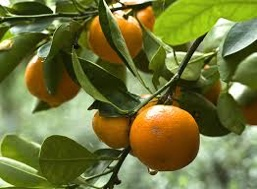
\includegraphics[width=0.5\textwidth]{sintesi/image7}
	\end{minipage}
\begin{tasks}
	\task Escriu la funció que relaciona el sou en \euro\ \ i els kg de taronges recollits 
	\task  Si el mes passat va cobrar 1230 \euro\ \, quants kg de taronges va recollir?
\end{tasks}
	\answers{  a)  $y=3x+600$;  \par  b) $\mathrm{1230}\mathrm{\ }=3x+600$   $\rightarrow$  $x=210$ kg de taronges}
	  
	
		\exer[2]  Representa gràficament les funcions
		\begin{tasks}(3)
			\task  $y=\ 2x$ 
			\task $y=x^2+1$
			\task $y=-x+3$
		\end{tasks} 
	\answers{ a) Lineal creixent; \quad b) paràbola còncava, $V(0,1)$; \quad Lineal decreixent}

\exer[2]  El següent gràfic mostra la variació de la velocitat d'un ciclista:
\begin{center}
	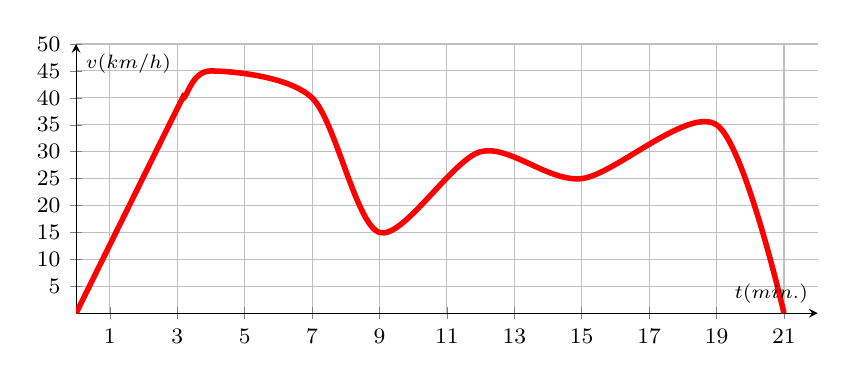
\begin{tikzpicture}[]
	\begin{axis}[width=11cm,height=5cm, axis background/.style={fill=white}, axis lines=middle, 
	grid = major,
	xlabel=$\scriptstyle t (min.)$,
	ylabel=$\scriptstyle v (km/h)$, 
	xtick={1,3,...,21},
	ytick={0,5,...,50},
	ymin = 0,
	ymax = 50,
	xmin = 0,
	xmax = 22,
	tick label style={font=\footnotesize},
	legend style={font=\normalsize,legend pos=south east},]
	\addplot[red, smooth, line width=2pt]  coordinates {(0,0) (3,38)   (3.2,40) (4, 45) (7, 40) (9,15) (12, 30)  (15, 25) (19, 35) (21, 0)};
	\end{axis}
	\end{tikzpicture}
\end{center}

\begin{tasks}
	\task Indica els intervals de creixement i decreixement.
	\task En què minuts va córrer a 10 km/h?
	\task Quina va ser la velocitat màxima i en quin minut passa? I mínima en ple trajecte?
	\task Quines altres característiques pots indicar sobre el gràfic?
\end{tasks}
\answers[cols=1]{[Creix a (0,\,4) i (9,\,12) i (15,\,19) min.; Decreix a (4,\,9) i (12,\,12) i (19,\,21) min., 1 min; 20.5 min, Màxim 45 km/h als 4 minuts i Mínima de 15 km/h als 9 min., És una funció contínua. El domini és (0,\,21) i el recorregut (0,\,45) ]}
	
\exer[2] Tenim una fotografia mida $10 \times 15$ que volem dibuixar sobre un quadre de mida $15P = 65 \times 50$. Justifica si serà possible encaixar tota la fotografia sense deformar-la. Si no és possible, explica quina part de la fotografia quedaria sense dibuixar.
\answers{No perquè $\dfrac{15}{10} \neq\dfrac{ 65}{60}$. Només podríem dibuixar 13 cm dels 15 cm de la fotografia.} 	
	
	
\exer[2]  En un triangle de costats 4 cm, 6 cm i 8 cm, calculau l'altura sobre el costat major. \textit{Ajuda:} Aplicau el teorema de Pitàgores i plantejau una equació.
\answers{$h=2,9$ cm}

\exer[2] Calcula l'àrea de la part pintada de les figures següents
\begin{tasks}(3)
	\task 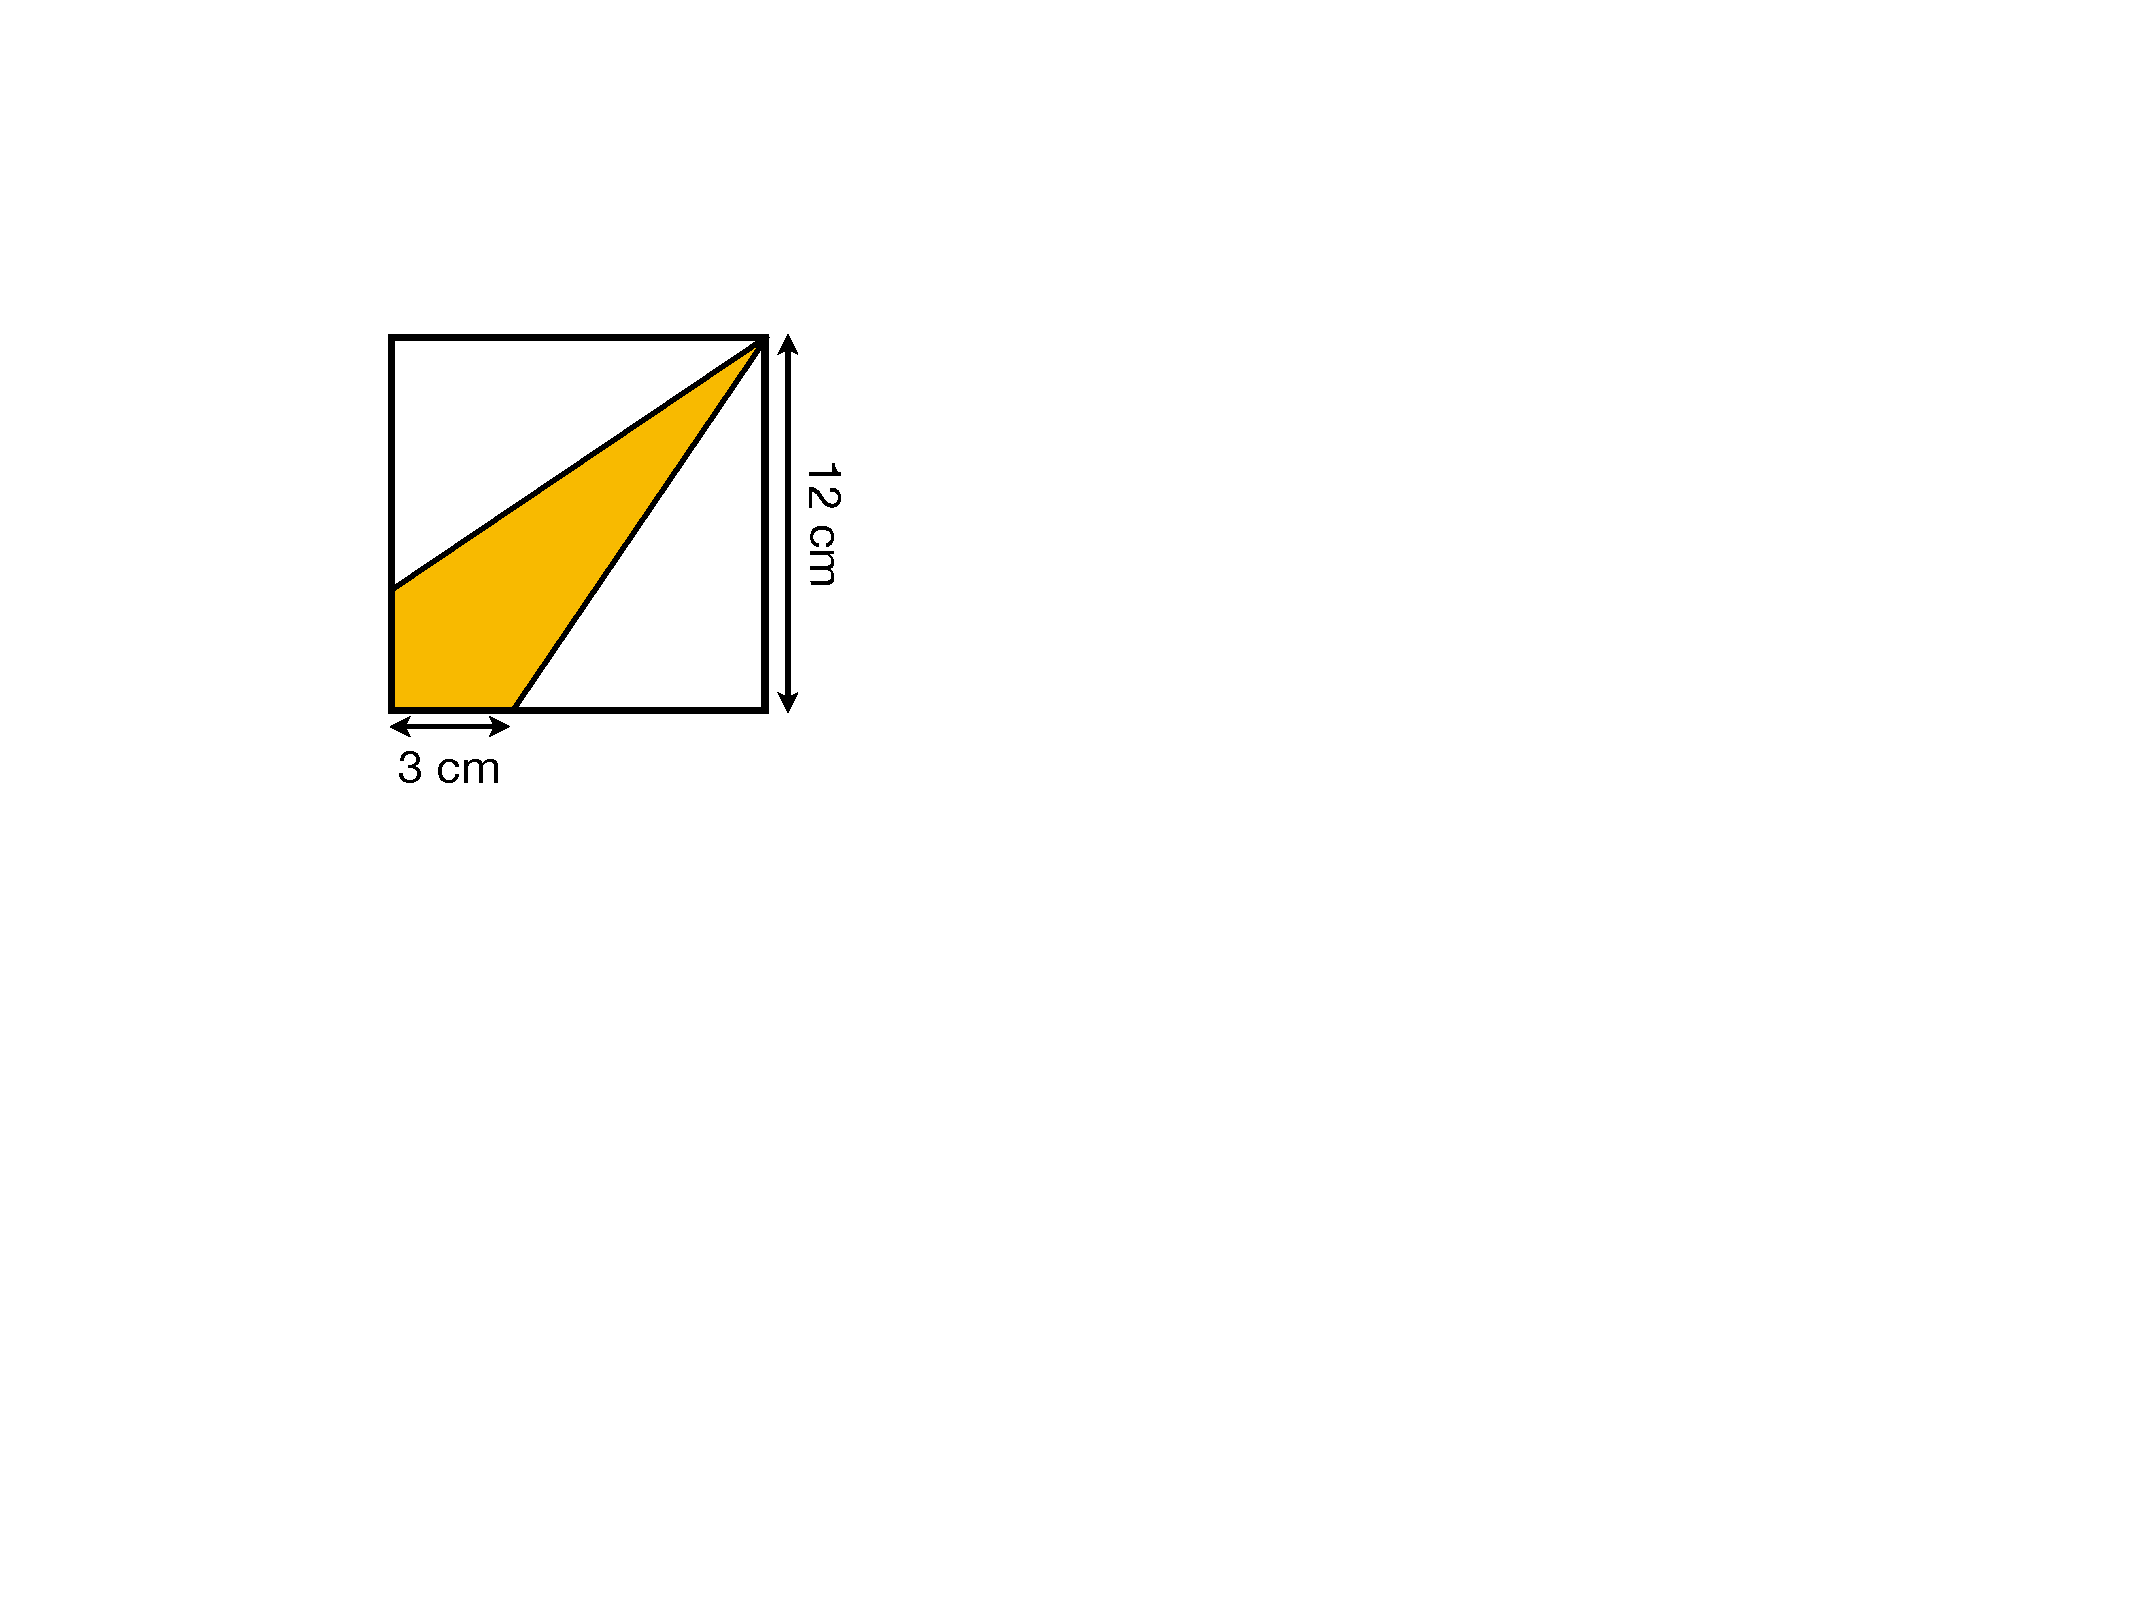
\includegraphics[width=0.2\textwidth, page=1]{sintesi/arees}
	\task \includegraphics[width=0.2\textwidth, page=2]{sintesi/arees}
	\task \includegraphics[width=0.2\textwidth, page=3]{sintesi/arees}
\end{tasks}
\answers{$A=36$ cm$^2$, $A=32$ cm$^2$, $A=377$ cm$^2$}


\exer[2] Dibuixa en el teu quadern un triangle amb vèrtexs $A(1, 2)$, $B(2, 0)$ i $C(3, 4)$. Troba els vèrtexs de les figures segons les transformacions:
\begin{tasks}
	\task Una translació de vector $\vec t(3,-2)$
	\task Una simetria d'eix OX
	\task Una rotació de centre O(0,0) i angle 90$^\circ$.
	\task Una simetria que té per eix la recta que passa pels punts $P(3, 4)$ i $Q(7, 0)$.
\end{tasks}
\answers[cols=1]{[$A'(4,0)$ $B'(5,-2)$  $C'(6,2)$, $A'(1,-2)$ $B'(2,0)$ $C'(3,-4)$, $A'(-2,1)$ $B'(0,2)$ $C'(-4,3)$, $A'(5,6)$ $B'(7,5)$ $C'(3,4)$]}

\exer[2] La piràmide de Kheops és una piràmide de base quadrangular de 230 m d'aresta i 147 m d'altura. Calcula l'àrea total i el volum d'aquesta piràmide. Dóna les respostes en hm$^2$ i hm$^3$.
\answers{$A_T =13,88$ hm$^{2}$, $V=2,59$ hm$^3$}

\vspace{-1.5cm}
\exer[2]\begin{minipage}[t]{0.7\textwidth}
Troba l'àrea total d'un prisma de base hexagonal de costat 6 cm i d'altura 10 cm. Calcula també el volum del prisma.
\end{minipage}
\begin{minipage}{0.3\textwidth}
	\centering
	\vspace{1.5cm}
	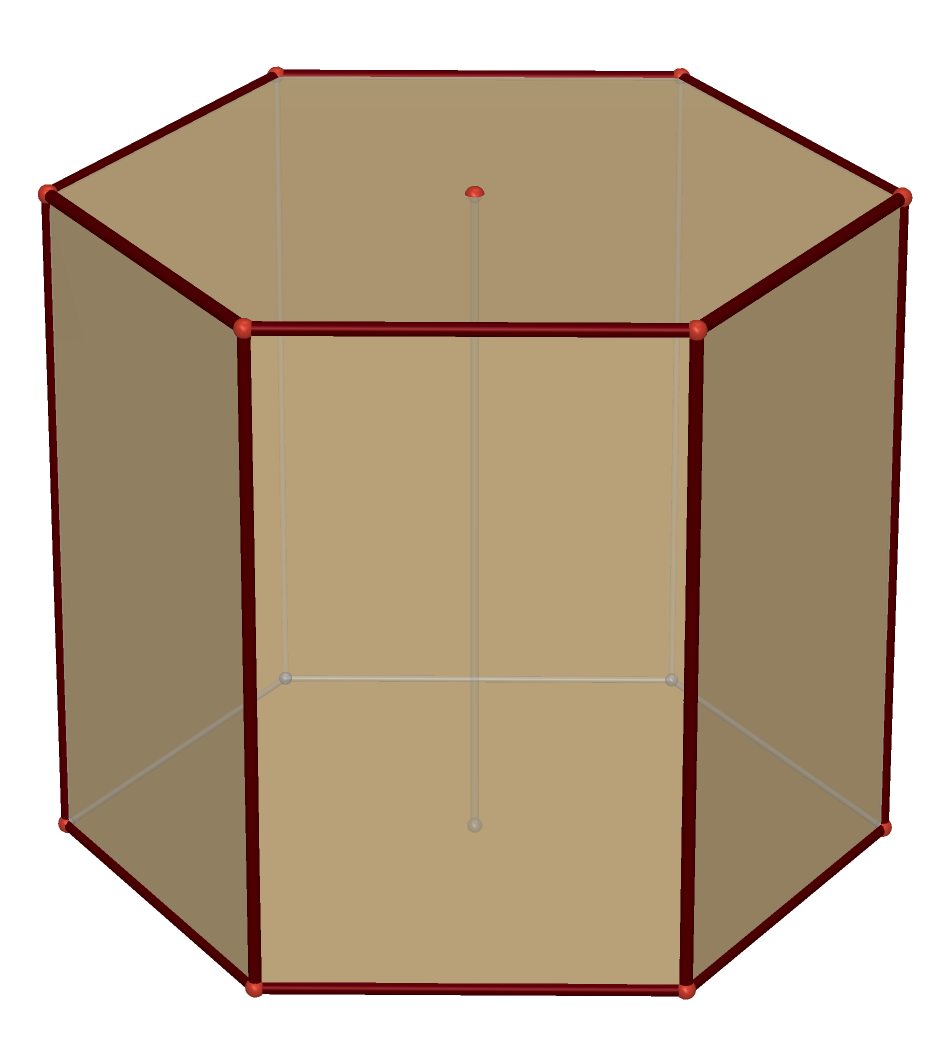
\includegraphics[width=0.5\textwidth]{img11/prisma-hexagonal}
\end{minipage}
\answers{$A_T =547,06$ cm$^{2}$, $V=935,3$ cm$^3$}	
 
 
\vspace*{-1.5cm}
\exer[2]\begin{minipage}[t]{0.7\textwidth}
	 Hem truncat un cub d'aresta 10 cm segons el pla ratllat de la figura. Calcula la superfície de la cara ratllada i el volum del cos.
\end{minipage}
\begin{minipage}{0.3\textwidth}
	\centering
	\vspace{1.5cm}
	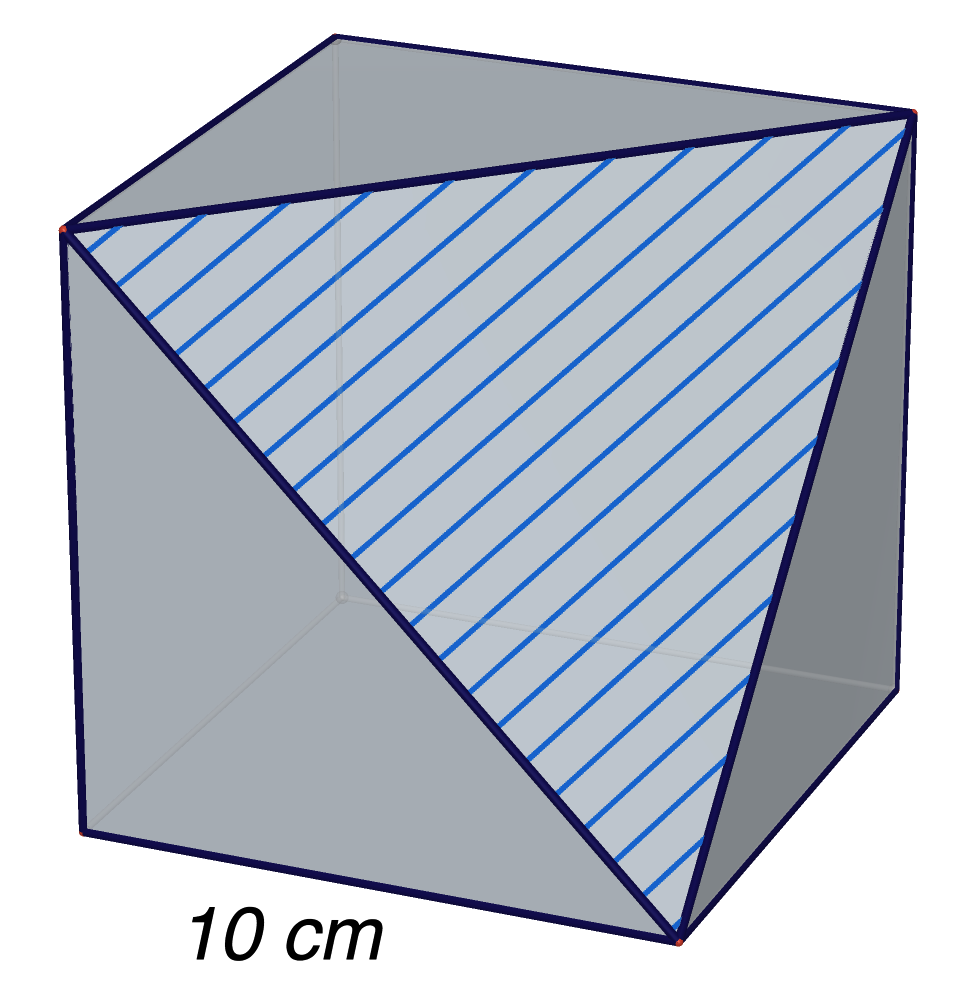
\includegraphics[width=0.5\textwidth]{sintesi/cubtruncat}
\end{minipage}
\answers{$A=50\sqrt{3}$ cm$^{2}$, $V=V_{cub} -V_{piram}=250$ cm$^{3}$}	
	
	
	
\exer[2] Tenim 3 pilotes de tenis dins d'una caixa cilíndrica de 6,6 cm de diàmetre en la que encaixen perfectament. Calcula el volum de la part buida.
\begin{center}
	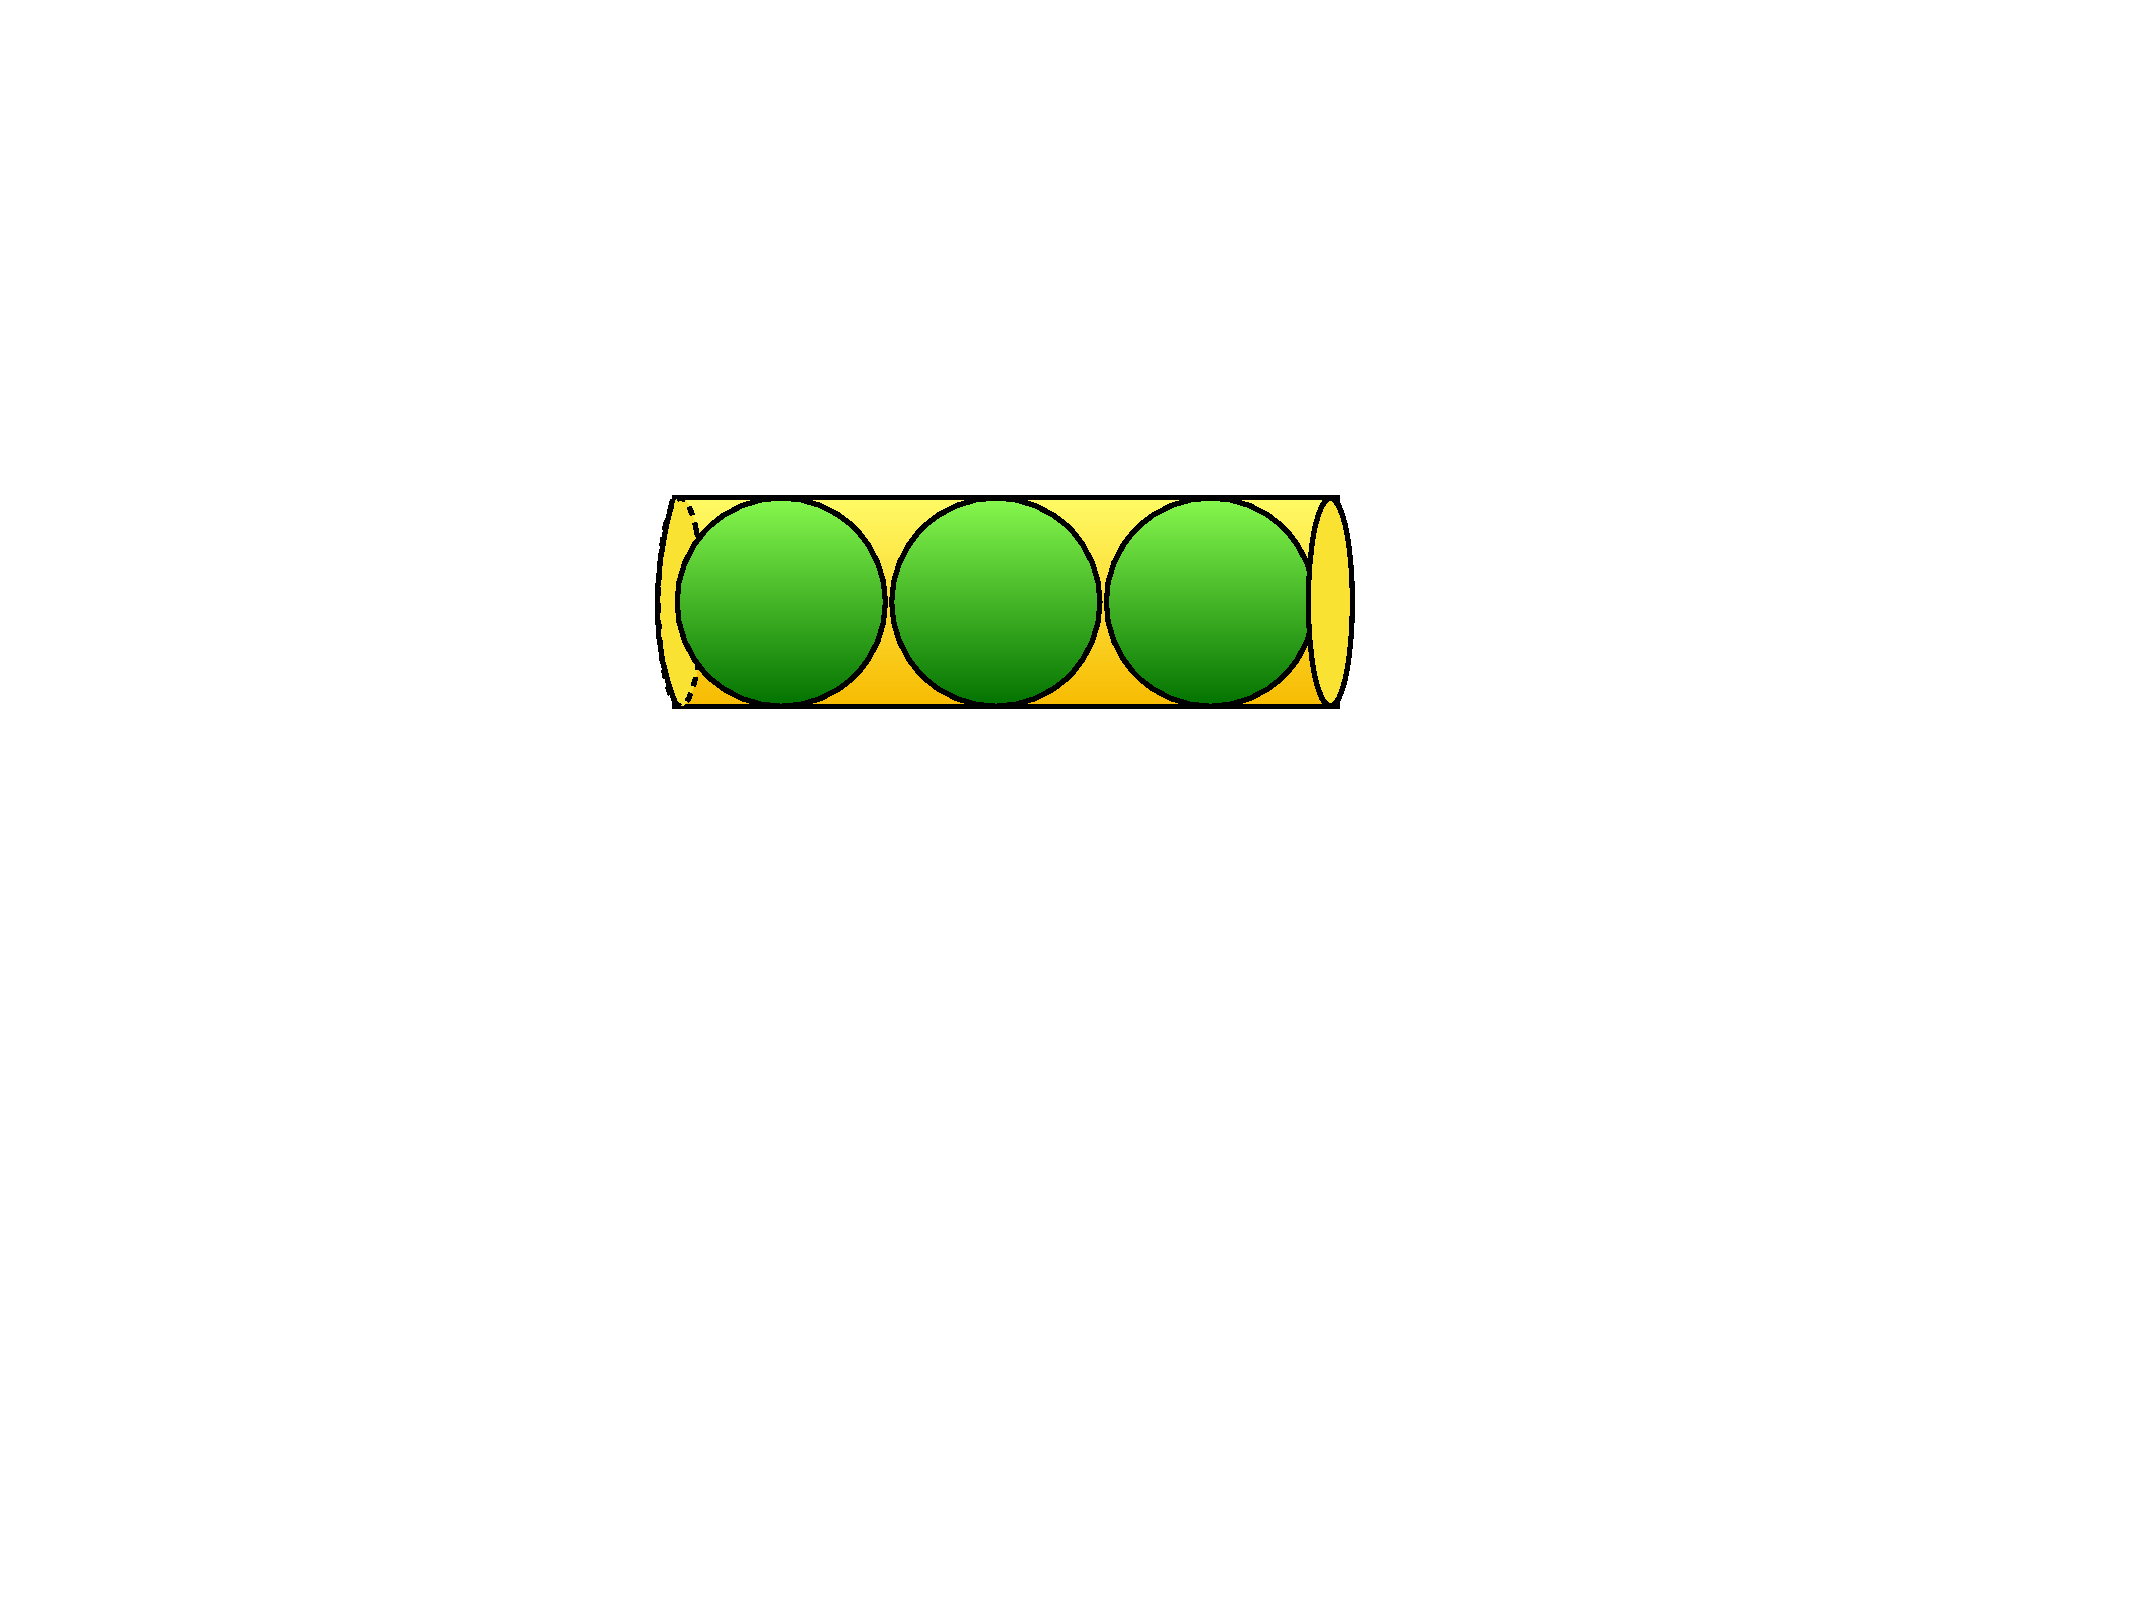
\includegraphics[width=0.35\textwidth]{sintesi/tennis}
\end{center}	
\answers{$V=338,7$ cm$^3$}

\exer[2] Una piscina té forma d'ortoedre de dimensions $8\times 4 \times 2 $ m. Hem fet una lectura del pH de l'aigua de 6.8. Les recomanacions pel bany són que el pH estigui al voltant de 7.2. Per això, haurem afegir augmentador del pH del qual mostram l'etiqueta d'instruccions a la figura. Quina quantitat de producte haurem de posar per obtenir el pH desitjat?   
\begin{center}
	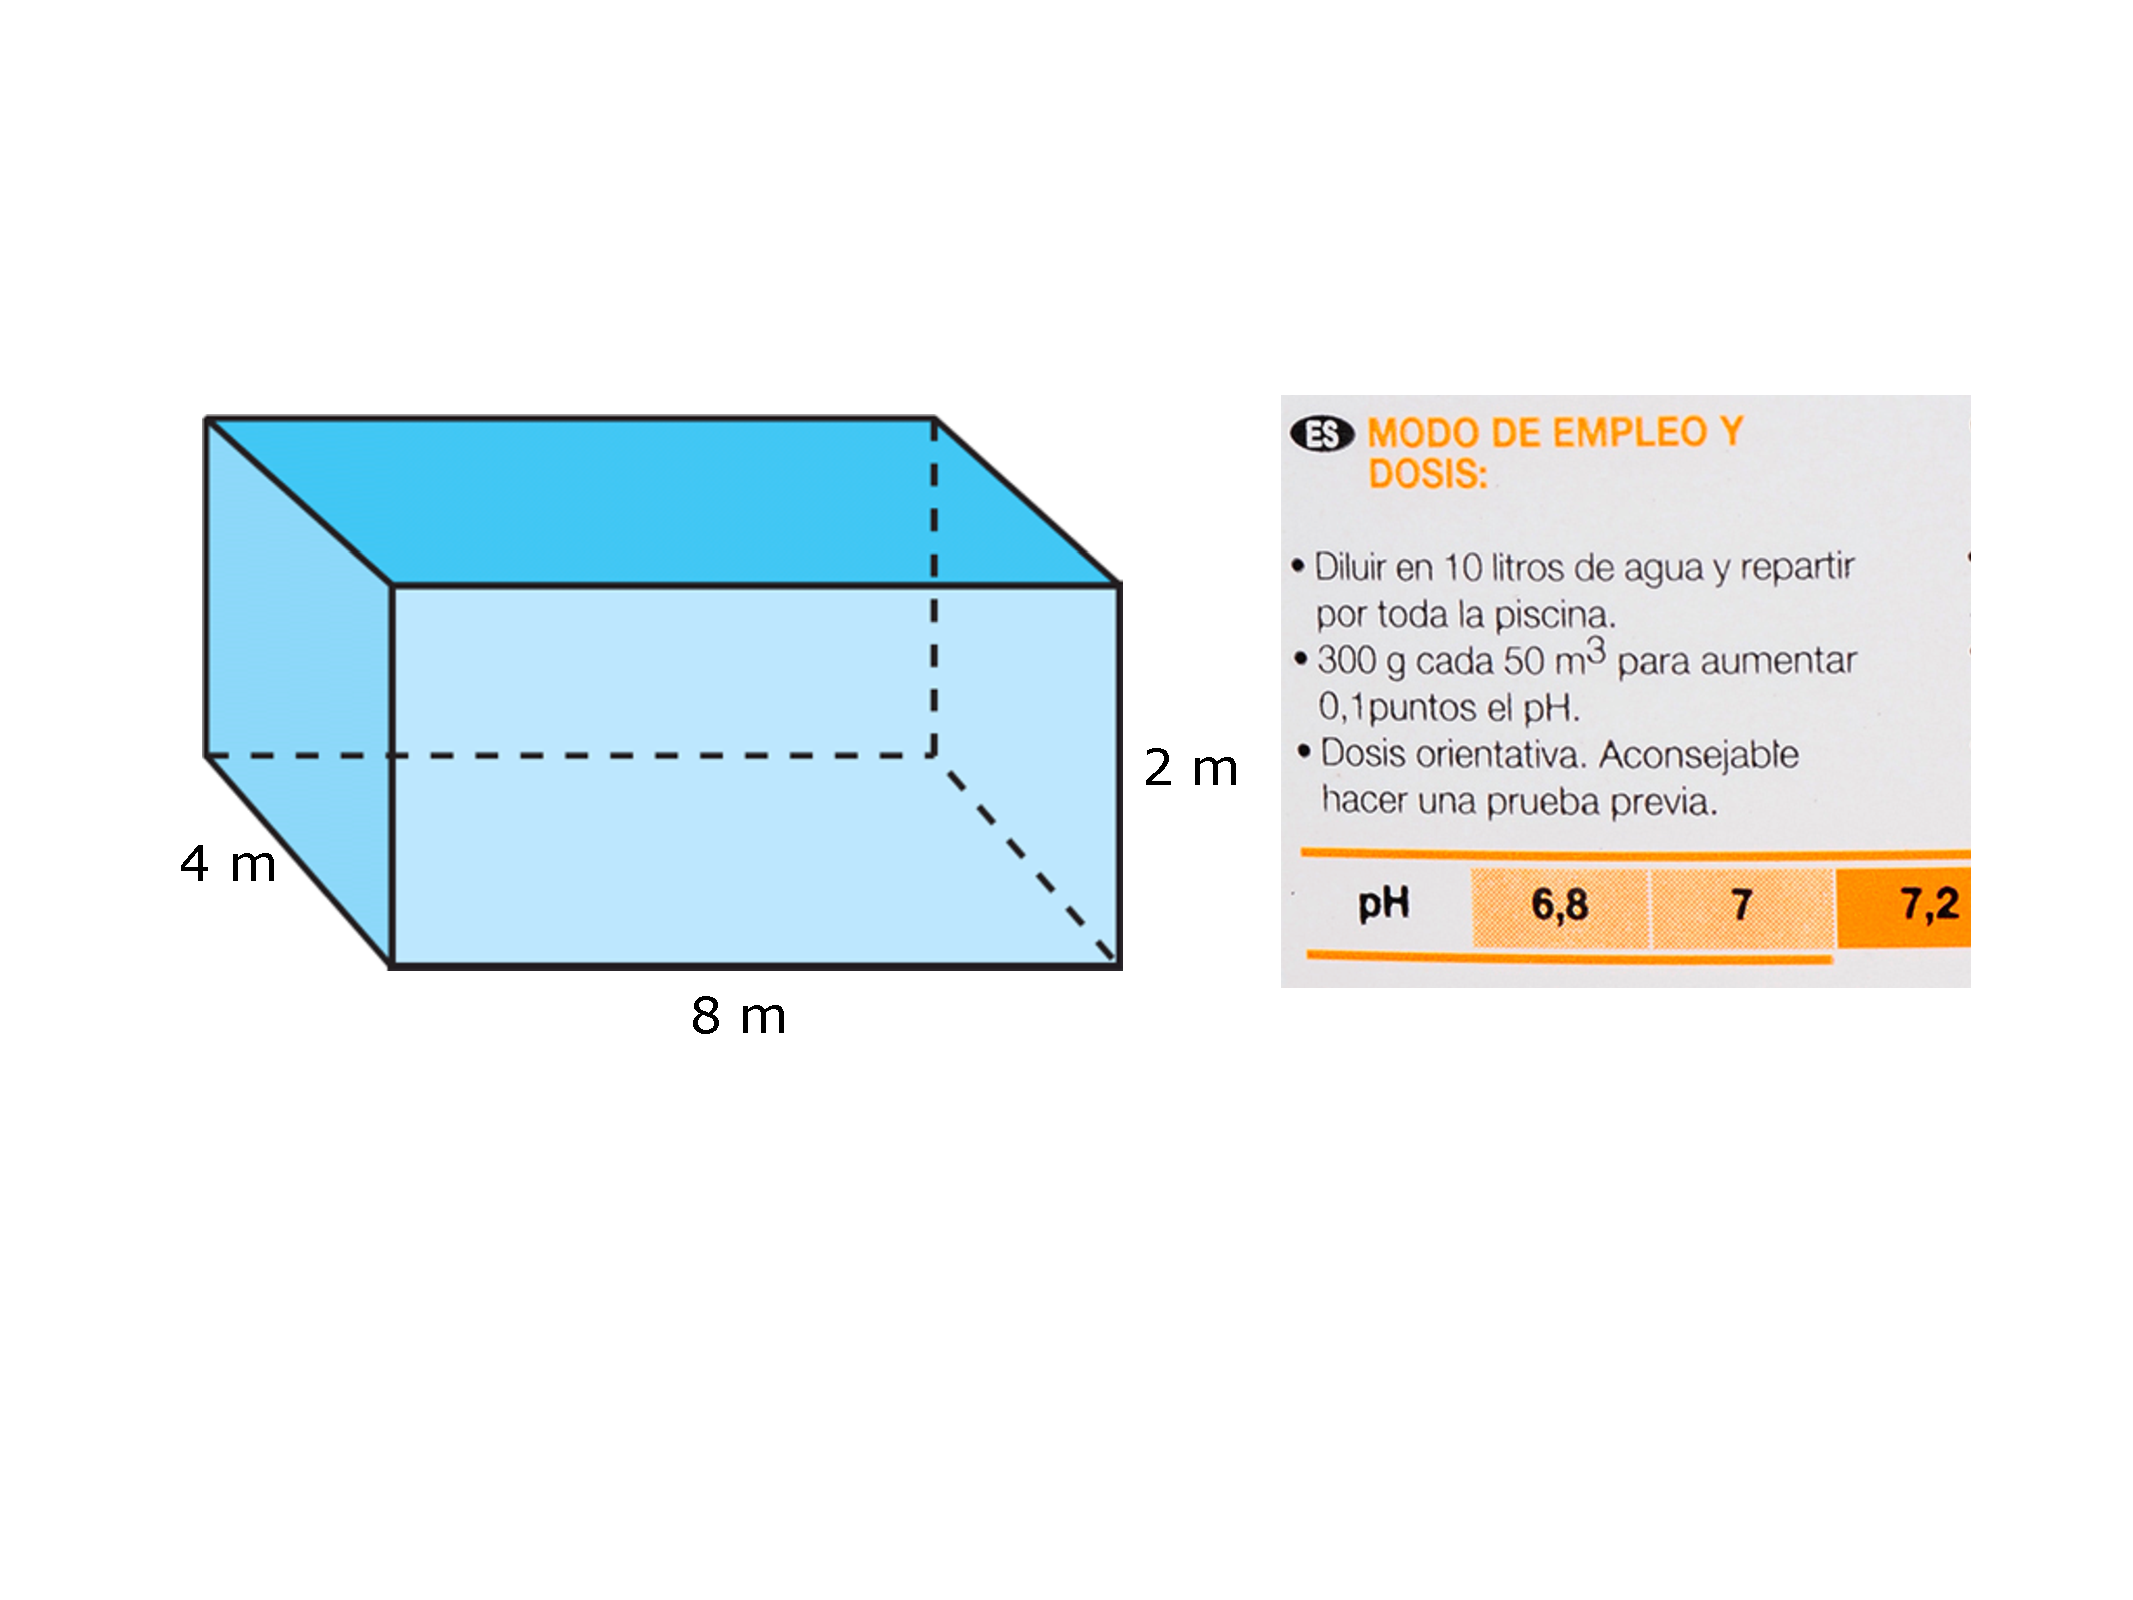
\includegraphics[width=0.75\textwidth]{sintesi/phmas}
\end{center}	
\answers{Hem de posar 1.54 kg de pH+ per augmentar 0.4 punts.}


 \end{mylist}

	
 
	